\documentclass[math,code]{amznotes}
\setcounter{tocdepth}{2}  % Only show sections in the ToC
\usepackage[utf8]{inputenc}
\usepackage{amsmath}
\usepackage{amsfonts}
\usepackage{graphicx}
\usepackage{tikz}
\usepackage{etoolbox}
\usepackage{tabularx}
\usepackage{float} % Needed for [H] placement specifier
\usepackage{wrapfig} % Needed for wrapping figures
\usepackage{diagbox} % For diagonal split in table
\usepackage{booktabs} % For better table formatting
\usepackage{hyperref} % For hyperlink
\usepackage{epigraph} % Used for quotes
\usepackage{xeCJK} % Used for Chinese Characters

\graphicspath{ {./images/} }
\geometry{
    a4paper,
    headheight = 1.5cm
}

\patchcmd{\chapter}{\thispagestyle{plain}}{\thispagestyle{fancy}}{}{}

\theoremstyle{remark}
\newtheorem*{claim}{Claim}
\newtheorem*{remark}{Remark}
\newtheorem{case}{Case}

\begin{document}
\fancyhead[L]{
    CDE2501 Sustainable Systems for Liveable Cities
}
\fancyhead[R]{
    Lecture Notes
}
\tableofcontents

\chapter{Tutorials}

\section{Tutorial 1}

\subsection{Project Methodology}

In this course, the project methodology is shown as follows:

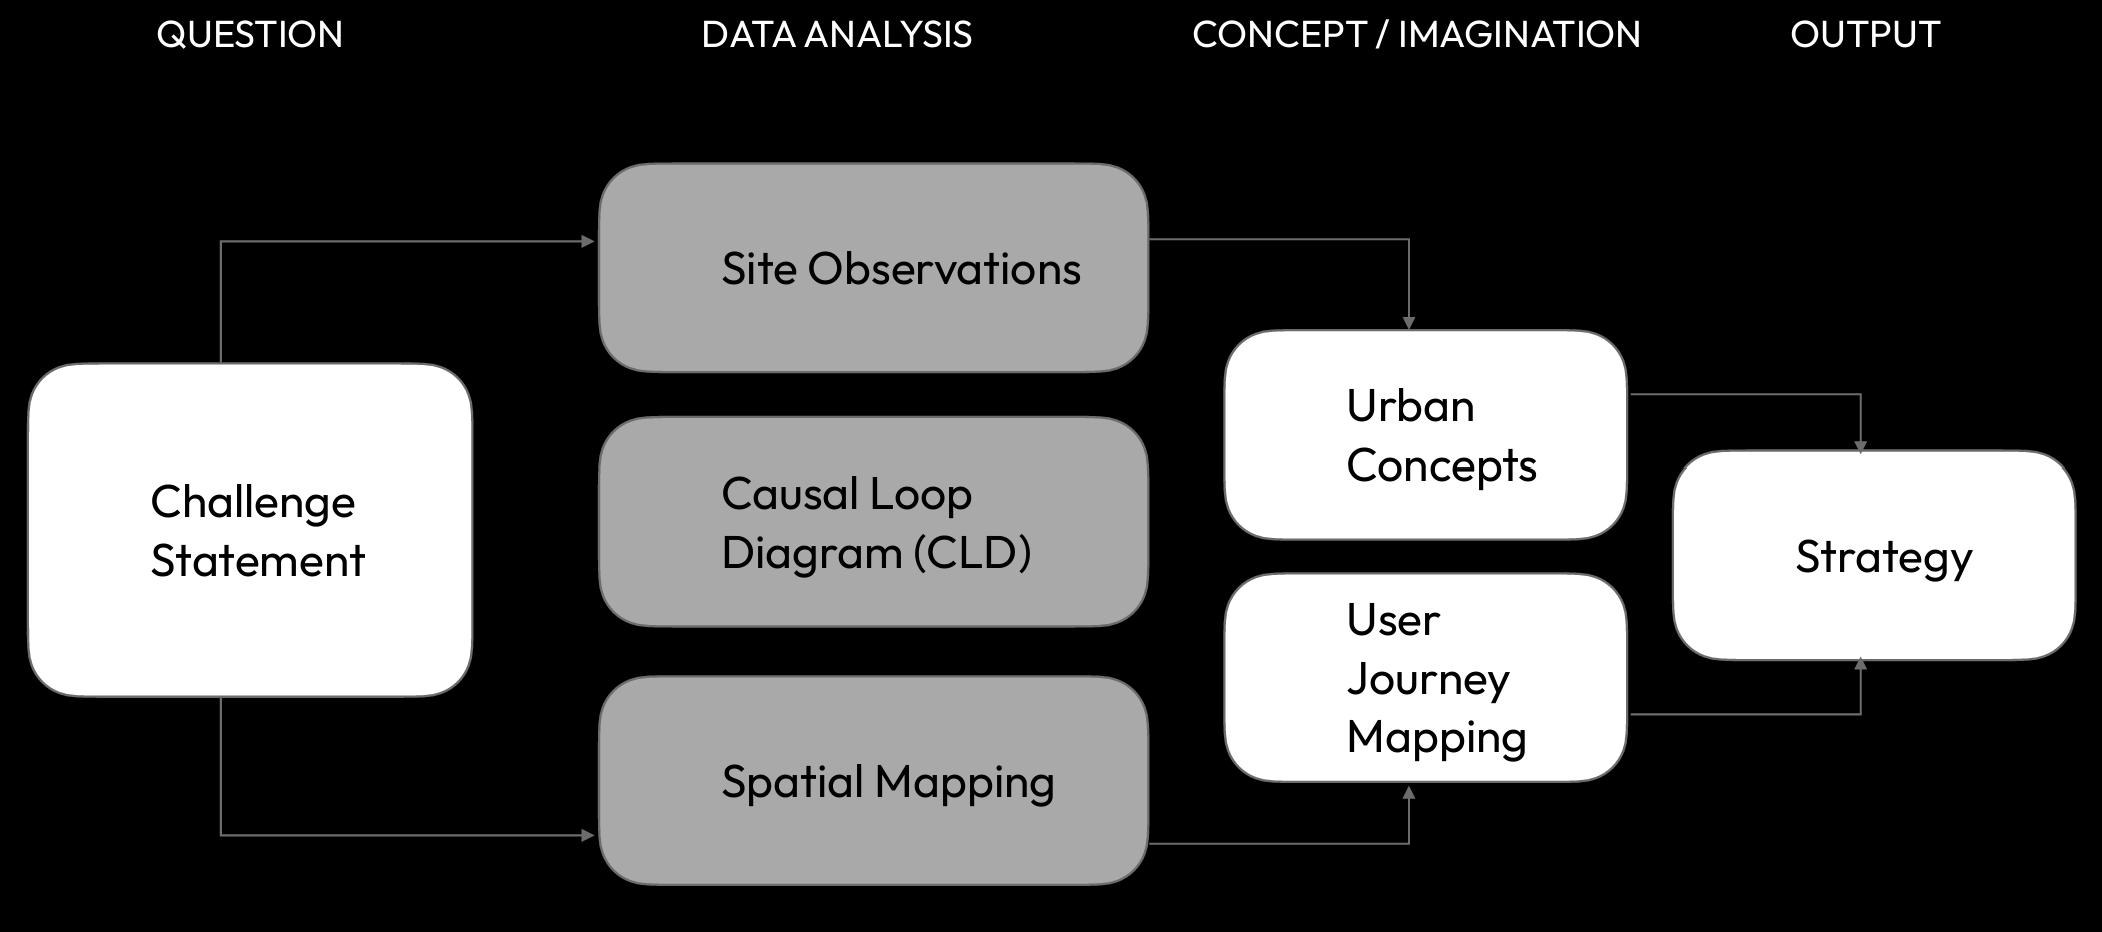
\includegraphics[width=1\linewidth]{images/project-methodology.png}

\subsection{Challenge Statement}

To form a challenge statement, we should use \textbf{Approach + Outcome + Strategy}. The outcome can be either \textbf{social} or \textbf{urban} outcome and the \textbf{strategy} can be sometimes replaced by \textbf{target demographic} also.

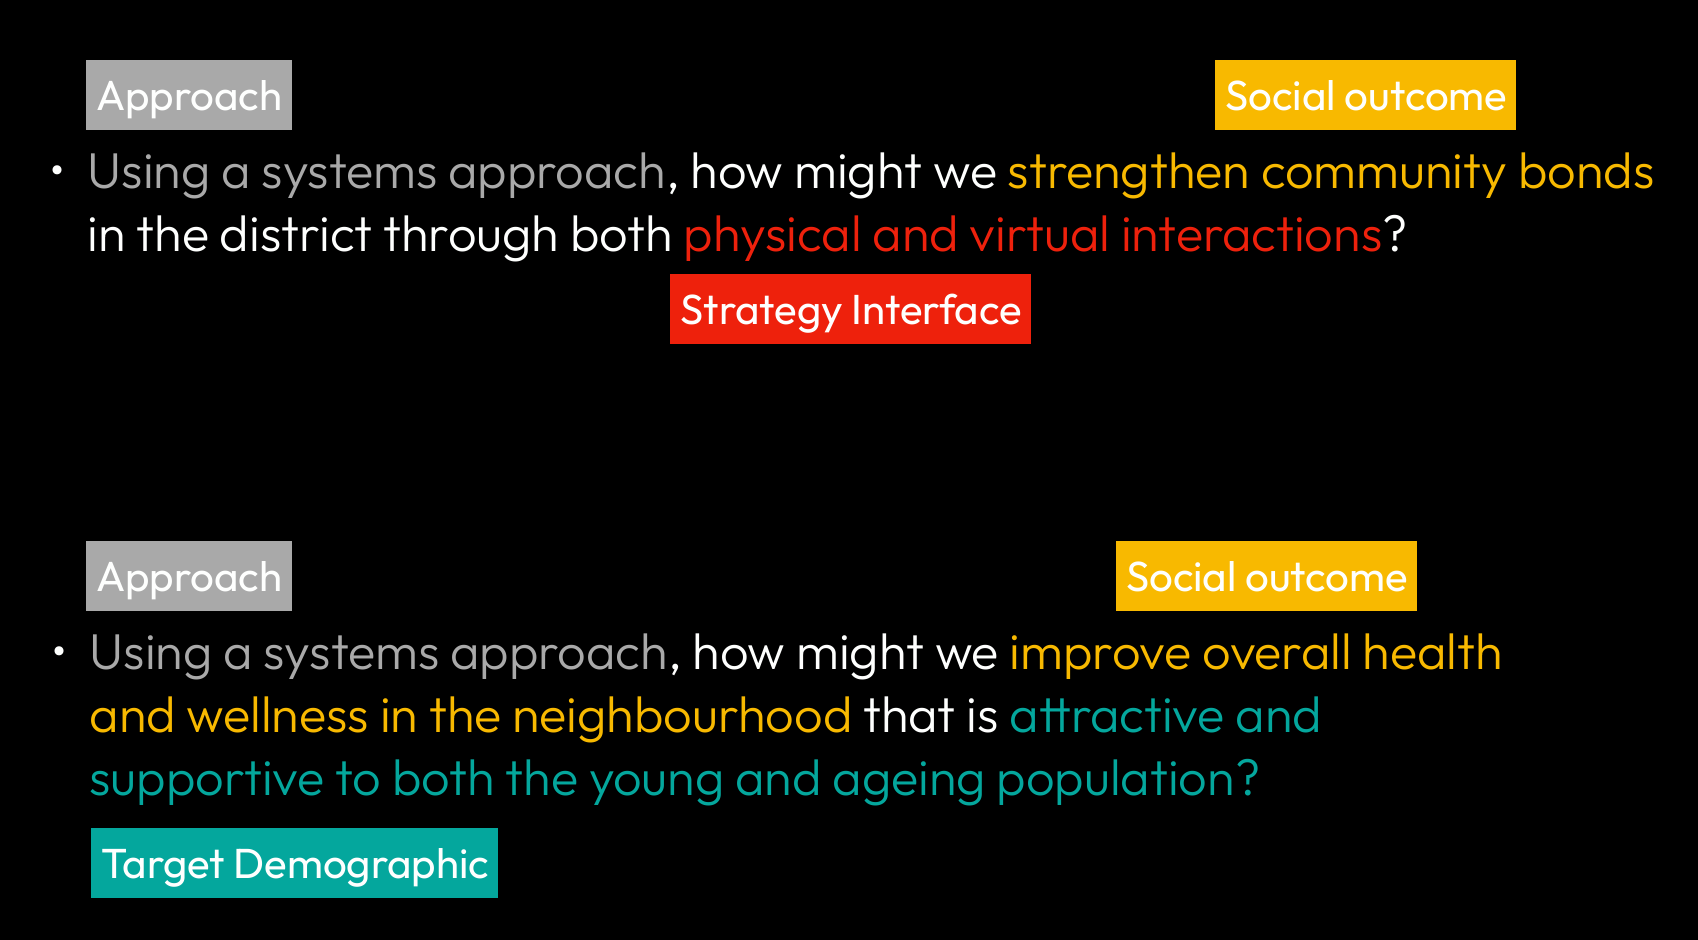
\includegraphics[width=1\linewidth]{images/challenge-statement-1.png}

\subsection{Casual Loop Diagram}

\subsection{Livability Framework}

The Liveability Framework consists of three key Liveability Outcomes (High Quality of Life, Competitive Economy and Sustainable Environment), which are achieved through three key underlying Systems (Integrated Master Planning and Development, Dynamic Urban Governance, Collaborative Ecosystem).

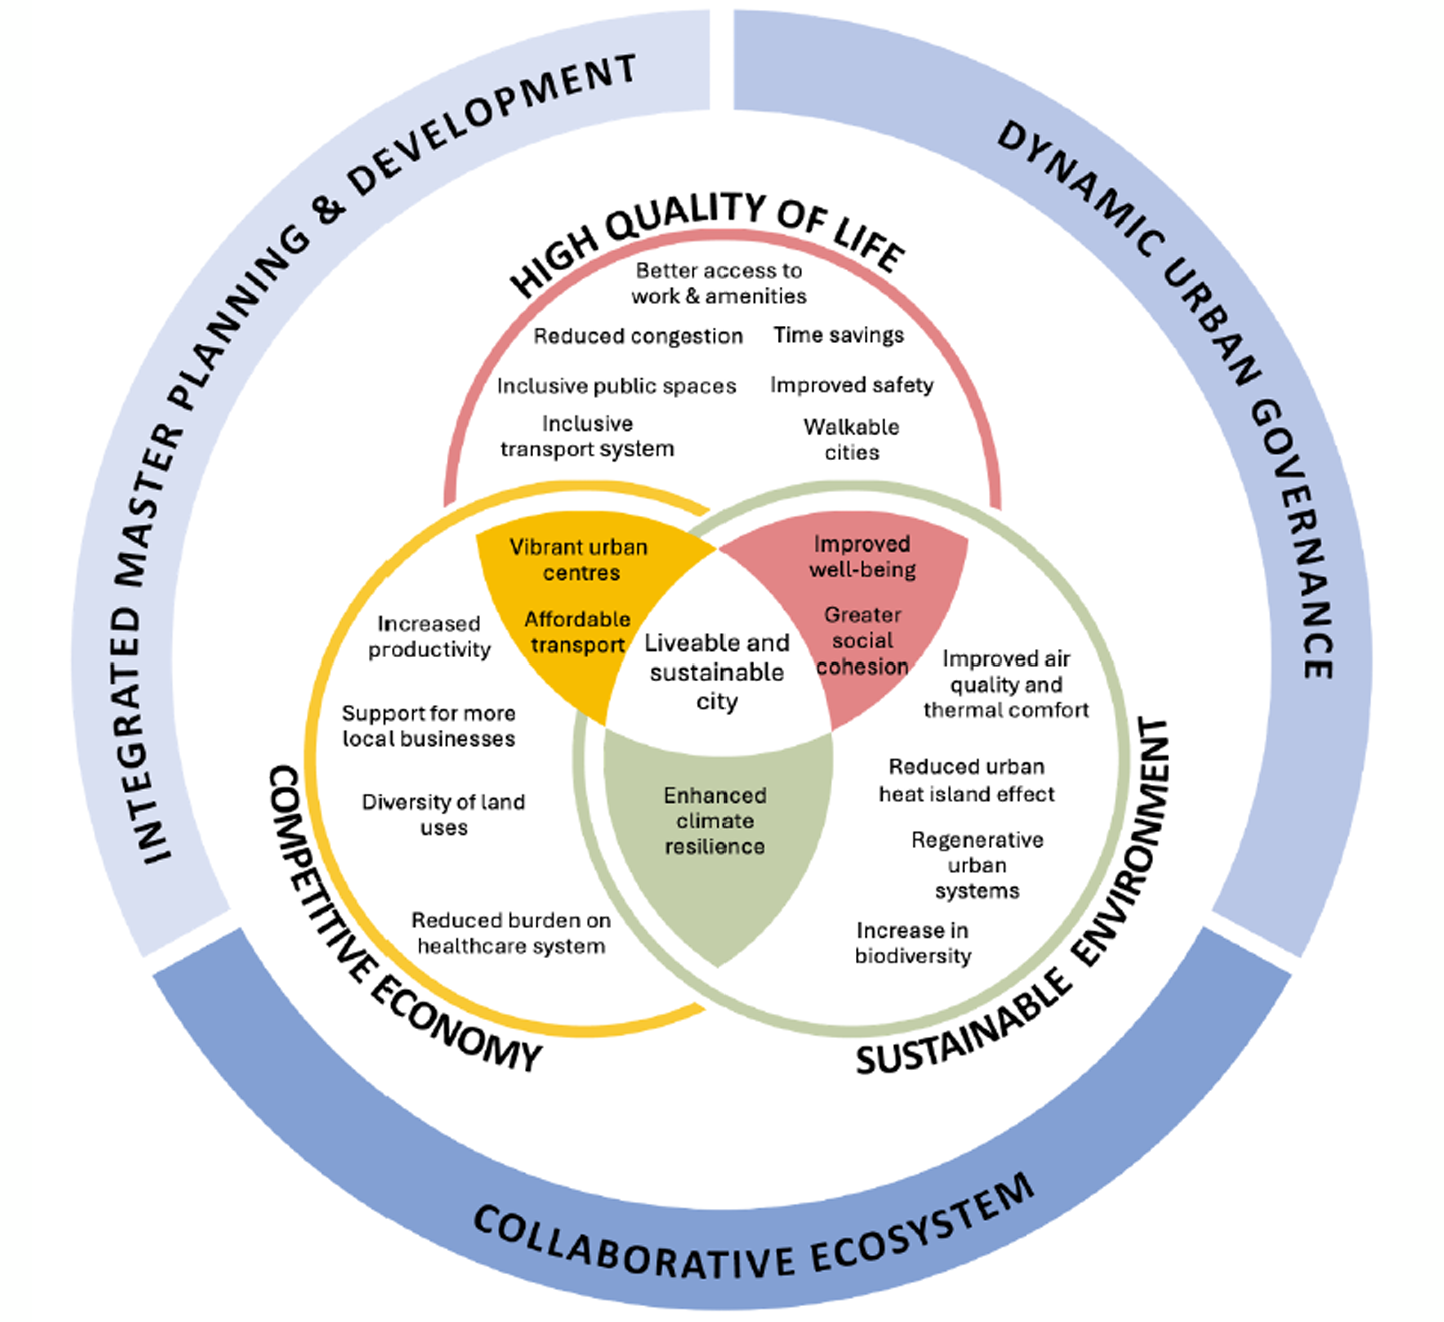
\includegraphics[width=1\linewidth]{images/livability-framework.png}

The link between the framework and CDE2501 is that

\begin{itemize}
    \item The three \textbf{Liveability Outcomes (High Quality of Life, Sustainable Environment, Competitive Economy)} become the standards by which you assess whether the site you are investigating has achieved these outcomes. Problems are the gaps between the ideals of the Liveability Outcomes and the current state of the site.
    \item The three underlying \textbf{Systems (Integrated Master Planning \& Development, Dynamic Urban Governance, Collaborative Ecosystem)} are not directly related to your project, as your project will deal with the scale of a neighbourhood or district rather than a whole city. But the following ideas behind these Systems will be applicable to your project: 
    \begin{itemize}
        \item Urban problems are complex due to the multiple causes and systems underlying them and this requires an integrated approach. The use of \textbf{casual loop diagram}.
        \item Any urban issue has multiple stakeholders, whether from government, private sector, or public, and these need to be considered and engaged in the process of developing solutions – this is both a dynamic process (as proposed solutions have to change with the input/consideration of these stakeholders) and a collaborative process (capitalising on the knowledge that the community and the private sector have about the realities on the ground) 
        \begin{itemize}
            \item Understanding the problem
            \item Coming up with solutions
            \item Evaluating your solutions
        \end{itemize}
    \end{itemize}
\end{itemize}

\subsection{The 3 Urban Concepts}
\subsubsection{Active Frontage}

The difference between active frontage and blank frontage can be summarized in the following figure clearly,

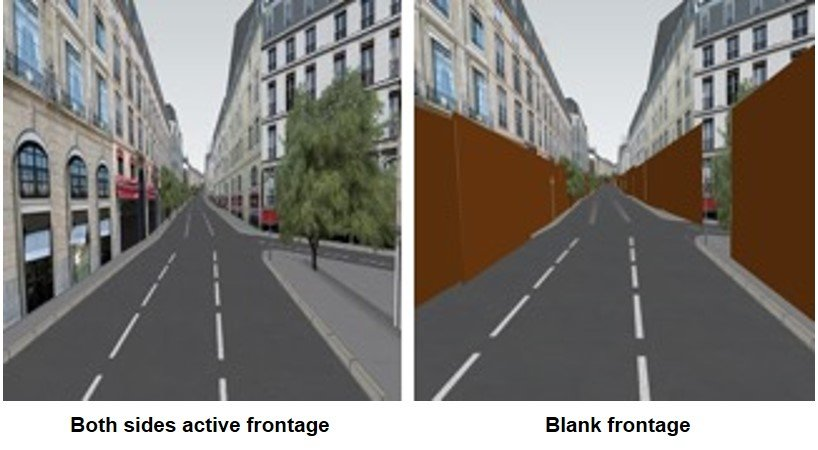
\includegraphics[width=1\linewidth]{images/active-frontage-example.png}

\end{document}
